\chapter{Servidor}
% Java - REST - JSON - JSOUP 
% Anexo 1 = HTML disciplinas material de apoio
% Anexo 2 = HTML material de apoio

Com o objetivo de extrair e preparar as informações a serem consumidas pela aplicação móvel do sistema acadêmico Minha Uno, foi desenvolvido em linguagem Java um servidor REST para facilitar e agilizar a extração dos dados. 

Utilizando-se da biblioteca \emph{jsoup} para a extração das informações e após o tratamento dos dados gerando-se arquivos JSON transmitidos utilizando um servidor REST, serão detalhadas nas próximas sessões o funcionamento de cada etapa da extração, preparação e transmissão das informações desde o sistema acadêmico Minha Uno até a aplicação móvel.

\section{Ferramentas Utilizadas}
Para o desenvolvimento do servidor foram utilizadas apenas ferramentas Open-Source, sendo que a linguagem escolhida para o desenvolvimento foi o Java, devido a quantidade de documentação encontrada na internet, e também por possuir bibliotecas prontas que permitem a extração, tratamento e disponibilidade das informações, facilitando assim a implementação do servidor.

\section{Extração das Informações}

Segundo informações obtidas da diretoria de Ti da Unochapecó, a instituição não possui um webservice com as informações do sistema acadêmico, e desta forma as informações exibidas na página são extraidas diretamente de uma coleção de banco de dados, o que tornaria inviável a integração direta com estas bases. Com a excasses de alternativas, foi necessário extrair as informações diretamente da página do sistema acadêmico. Para todos os processos de extração foi utilizada a biblioteca \emph{jsoup}, sendo que a mesma é responsável pela conexão aos diferentes endereços do sistema acadêmico e pela extração das informações a partir do retorno das consultas de navegação, ou seja, sendo extraidas as informações a partir do HTML retornado pelo sistema acadêmico atual.

Após o devido tratamento utilizando-se filtros com expressão regular e outros comandos permitidos pelo \emph{jsoup}, as informações necessárias para a aplicação são obtidas, sendo que na continuidade do capítulo será explicado como cada grupo de informações foi extraido e posteriormente preparado para ser consumido pelos dispositivos móveis.

Todas as expressões utilizadas na biblioteca \emph{jsoup} podem ser testadas na página web \url{http://try.jsoup.org/} utilizando como entrada o código HTML da página a ser analizada. Mais informações sobre as expressões utilizadas podem ser obtidas em \url{http://jsoup.org/cookbook/extracting-data/selector-syntax}.

Como toda a extração é baseada no retorno do código HTML do sistema atual, qualquer alteração no layout do arquivo HTML retornado pela página do sistema acadêmico Minha Uno resultará em problemas na extração dos dados.


\subsection{Login}
Com o objetivo de validar se o login fornecido pelo usuário na aplicação é válido e extrair o cookie (identificador de sessão utilizado para as acesso as informações obtidas apenas pelo login válido do usuário), o servidor possuí como primeira tarefa ao receber uma solicitação da aplicação a validação de login.

Utilizando-se do método POST do HTTP, os dados de login são enviados utilizando o endereço \url{https://www.unochapeco.edu.br/usuarios/login?login_submited=1&usuario=USUARIO&senha=SENHA&submit=entrar} (as palavras USUARIO e SENHA devem ser substituidas pelas respectivas informações).

%\begin{algorithm}[H]
% \SetAlgoLined
% \KwData{Login e Senha do usuário}
% \KwResult{Cookie de sessão da conexão e indicação de login válido}

% \If{Não existe sessão armazenada}
% {
%  Obtém o identificador de sessão\;
% }
 
% Validação da validade do login com base nos elementos retornados pela página\; 
 
%\caption{Validação de login e captura de sessão}
%\end{algorithm}

%\begin{algorithm}
%\caption{Validação de login e captura de Cookie}
%\begin{algorithmic}[1]

%$var session \gets null$

%\Function{connect}{user, pass}
%  \If {$session = vazio$}
%    \State $session \gets identificador de sessão extraido utilizando jsoup$
%  \EndIf
  
%  \State \Return Cookie da da sessão
%\EndFunction
%\end{algorithmic}
%\end{algorithm}

O algoritmo de extração do cookie e validação do login não apresenta nenhuma complexidade, conforme pode-se observar no Algoritmo 1. Para a exemplificação dos algoritmos neste capítulo não será adicionado código fonte em java, exibindo-se trechos de pseudo-código com relevância para este trabalho.

%%% Aqui é a sessão de extração do material de apoio
\subsection{Material de Apoio}
Com o objetivo de extrair a relação dos materiais eletrônicos postados pelos professores em cada disciplina cursada pelo acadêmico. Para melhor entendimento, o algoritmo será dividido em duas partes, sendo que a primeira parte mostrará como são extraidas as informações referentes as disciplinas cursadas pelo acadêmico, e a segunda parte do como são extraidas as informações dos materiais disponíveis.

%Aqui ta o algoritmo q vc nunca acha Andrei!!!!
%O Algoritmo 2 mostra como as informações dos materiais são extraidas, e o mesmo será detalhado nos itens 5.2.2.1 e 5.2.2.2.

%%% Aqui é a subsubsessão de extração das disciplinas
\subsubsection{Extração das Disciplinas}
Com o objetivo de extrair a lista das disciplinas pertencentes ao módulo de material de apoio do sistema acadêmico, é necessário que a informação seja extraida a partir do código HTML retornado pela url \url{https://www.unochapeco.edu.br/saa/materialApoio.php}. Para a obtenção das disciplinas corretas cursadas pelo acadêmico, é utilizado o cookie de sessão capturado no momento do login, conforme explicado no item 5.2.1 deste trabalho. Um exemplo de código HTML retornado pelo servidor a partir deste tipo de consulta pode ser visto no anexo 1 deste trabalho.

Em posse do código HTML retornado e aplicando-se a expressão ``\emph{form tr td:eq(1) a}'' na biblioteca \emph{jsoup} sob o mesmo, obtém-se como retorno a lista das disciplinas cursadas pelo acadêmico, conforme pode ser visto na figura 5.

\begin{figure}[!htb]
     \centering
     \caption[Extração de Informações - Lista de Disciplinas do Material de Apoio]{Lista das disciplinas extraidas.}
     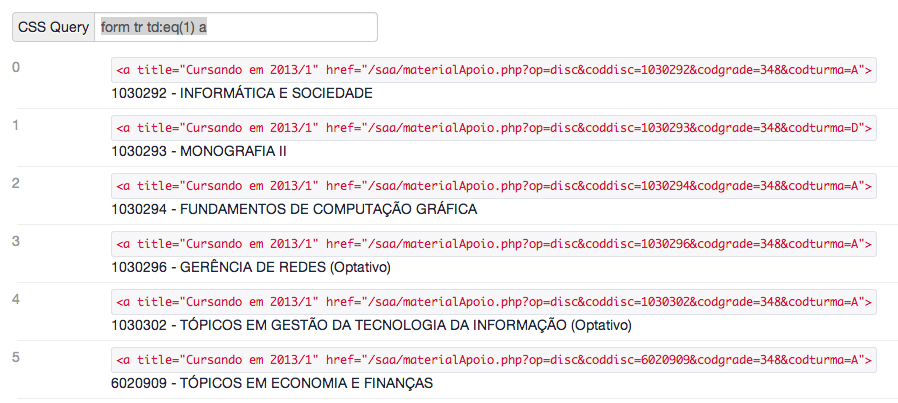
\includegraphics[scale=0.5]{imagens/listadisciplinasmaterialapoio.png}
     \\ Fonte: Do Autor.
\end{figure}

A partir da lista retornada acima, é possível retornar diretamente a disciplina no formato ``\emph{Código - Nome}''. Também como pode-se verificar na Imagem 5, acima do nome da disciplina é exibida a tag HTML completa, sendo que nesta tag pode-se verificar o atributo \emph{href}, que possui o caminho completo para serem extraidos os materiais da disciplina.

Após a extração do nome da disciplina e da tag \emph{href}, é necessária a extração das informações dos materiais da disciplina, explicada na sessão 5.2.2.2 deste trabalho.

%%% Aqui é a subsubsessão de extração dos materiais
\subsubsection{Extração dos Materiais}
Após a extração da lista de disciplinas e da referência ao endereço web onde as disciplinas podem ser acessadas, é necessário extrair as informações dos materiais propriamente ditos.

A partir do código HTML (disponível no anexo 2, sendo que o mesmo é pertencente a uma disciplina do 9º período de Ciência da Computação na grade 348) obtido pela url capturada (conforme explicado na sessão 5.2.2.1). No código retornado, existem 4 informações relevantes, sendo elas: nome, url, publicação e descrição.

Para a extração do nome do material, a expressão ``\emph{form tr:contains(Arquivo) a}'', sendo que a mesma retorna uma lista com o nome das disciplinas, conforme pode ser visto na Figura 6.

\begin{figure}[!htb]
     \centering
     \caption[Extração de Informações - Lista de Nomes dos Materiais de uma disciplina]{Lista de nomes dos materiais de uma disciplina.}
     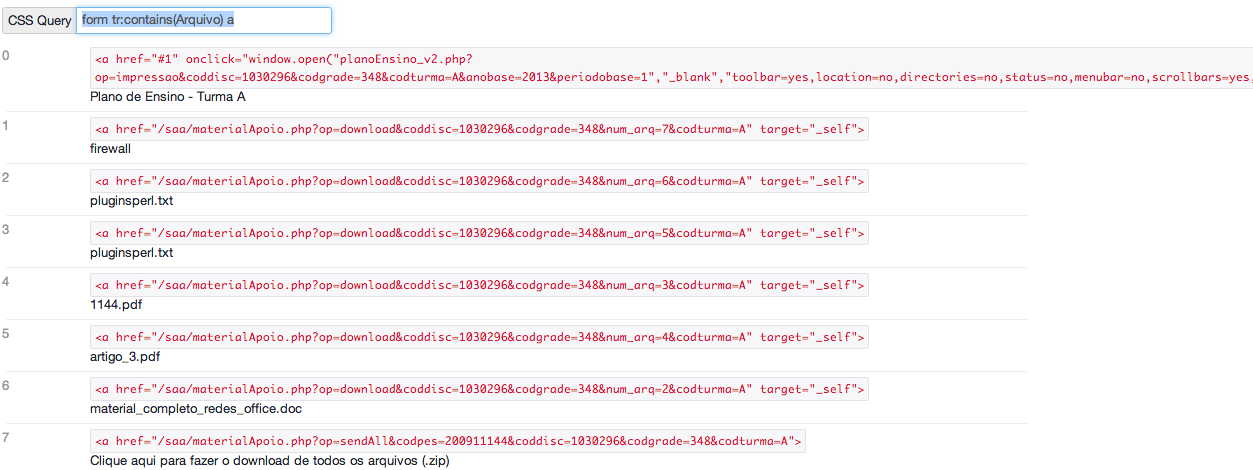
\includegraphics[scale=0.35]{imagens/listamateriaisdisciplinasnomematerial.png}
     \\  Fonte: Do Autor.
\end{figure}

Verificamos na Figura 6 que a mesma expressão retorna no campo principal o nome das disciplinas, e na sua referência (exibida em vermelho) o campo href, que nos é interessante para o acesso direto ao arquivo listado. Desta forma, utilizando-se da mesma expressão é possível extrair a url de acesso direto ao arquivo e também o nome do arquivo a ser acessado. Desta forma, duas informações já são preenchidas a partir da mesma consulta. 

Para obtermos a publicação, que nada mais é o nome do professor que postou o material e a data de postagem, utiliza-se a expressão ``\emph{form tr:contains(Publicação) td:eq(1)}'', e o seu retorno pode ser verificado na Figura 7.

\begin{figure}[!htb]
     \centering     
     \caption[Extração de Informações - Lista das publicações dos materiais]{Lista de publicação dos materiais de uma disciplina.}
     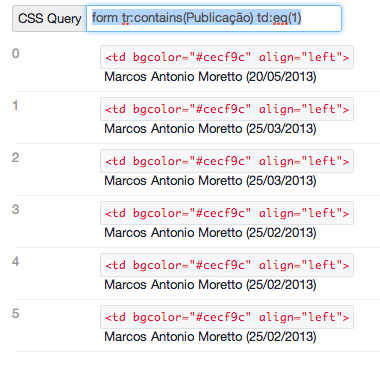
\includegraphics[scale=0.7]{imagens/listamateriaisdisciplinaspublicacao.png}
     \\  Fonte: Do Autor.
\end{figure}

Para obtermos a descrição dos materiais postados, a expressão ``\emph{form tr:contains(Descrição) td:eq(1)}'' onde obtém-se como resultado a lista da descrições dos materiais, confome pode ser visto na Figura 8.

\begin{figure}[!htb]
     \centering
     \caption[Extração de Informações - Lista das descrições dos materiais]{Lista de descrição dos materiais de uma disciplina.}
     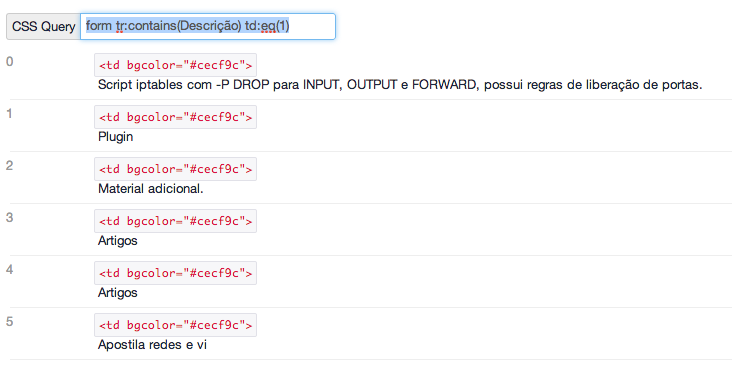
\includegraphics[scale=0.6]{imagens/listamateriaisdisciplinasdescricao.png}
     \\  Fonte: Do Autor.
\end{figure}

\newpage

\subsection{Notas da Graduação}
Com o objetivo de de extrair as avaliações e as respectivas notas das avaliações aplicadas aos acadêmicos, foi desenvolvida a classe de extração das notas da graduação. Para melhor entendimento, o algoritmo será dividido em três partes, onde a primeira representará a extração da lista de disciplinas cursadas pelos acadêmicos, a segunda as informações referentes as avaliações e notas das disciplinas em aberto e a terceira parte explicará a extração das disciplinas já finalizadas pelo acadêmico.

Assim como na sessão 5.2.2, será utilizada a biblioteca \emph{jsoup} para extração das informações, utilizando-se das mesmas recomendações da sessão mencionada anteriormente.

\subsubsection{Extração das Disciplinas}
Com o objetivo de extrair a lista das disciplinas pertencentes ao módulo de notas da graduação do sistema acadêmico, é necessário que a informação seja extraida a partir do código HTML retornado pela url \url{https://www.unochapeco.edu.br/saa/notas.php}. Para a obtenção das disciplinas corretas cursadas pelo acadêmico, é utilizado o cookie de sessão capturado no momento do login, conforme explicado no item 5.2.1 deste trabalho. Um exemplo de código HTML retornado pelo servidor a partir deste tipo de consulta pode ser visto no anexo 2 deste trabalho.


\subsubsection{Extração das Notas das Disciplinas em Aberto}

\subsubsection{Extração das Notas das Disciplilas Finalizadas}

\subsection{Horários do Semestre}


\section{Preparação dos Dados}

\section{Servidor REST}
